\documentclass[10pt]{article}
\usepackage[top=1cm, bottom=1cm, left=1cm, right=1cm]{geometry}
\usepackage{graphicx}
\usepackage[colorlinks=true]{hyperref}
\usepackage{verbatim}
\usepackage{enumerate}

\title{Wesnoth UMC Development \\ Developer's Manual}
\author{Timotei Dolean - \href{mailto:timotei21@gmail.com}{timotei21@gmail.com}}

\begin{document}

\maketitle

\tableofcontents
\setcounter{tocdepth}{3}
\newpage

\newcounter{cnt}
\newcommand{\icnt}{ \stepcounter{cnt} \thecnt }

\section{Foreword}
Through this readme the following terms with the specified meaning will be used:
\begin{enumerate}
\item Navigator - an Eclipse view that shows the projects in the workspace
\item Project - a directory on the harddrive that is represented as a top directory in the navigator.
\item Container - this is a directory or a project. Basically it can contain any file or directory children.
\end{enumerate}

The following image will highlight the terms used: 1 - Navigator, 2 - Project, 3 - Containers, 4 - Map files, 5 - Config files that contain WML code

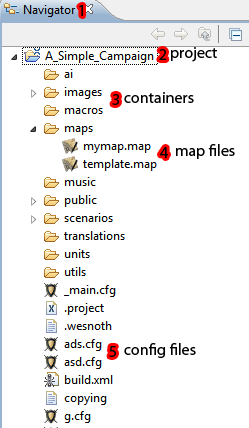
\includegraphics{definitions.png}

\section{Common prerequisites}
\begin{enumerate}
\item The plugin runs on the following platforms: Windows 32/64 bit, Linux 32/64 bit and Mac OSX 64bit. Note that \textbf{Mac OSX 32 bit} is \textbf{not supported}. If you want to know why, please consult the Frequently Asked Questions section.
\item Download and install Sun's Java Version 6 (Java SE6):
\begin{enumerate}
\item If you are going just to use the plugin (User): \href{https://cds.sun.com/is-bin/INTERSHOP.enfinity/WFS/CDS-CDS_Developer-Site/en_US/-/USD/ViewProductDetail-Start?ProductRef=jre-6u21-oth-JPR@CDS-CDS_Developer}{Download JRE}
\item If you are going to modify it or run it from source (Developer): \href{http://java.sun.com/javase/downloads/widget/jdk6.jsp}{Download JDK}
\end{enumerate}
\textit{Note:} The plugin uses Java SE6, thus older versions (like 1.4 or 1.5) don't work with it.\\
\textit{Note:} Please double check the java installed on your system. On some machines there is the OpenJDK or other Java versions. Use just Sun's so there will be no problems.
\item Download and install Python 2.x:
\begin{enumerate}
\item \textbf{Windows:} Download and install from here: \href{http://python.org/download/}{Download Python} , selecting a 2.x version
\item \textbf{Linux:} Use the regular package manager for installing it from the repositories.
\item \textbf{Mac:} Download and install from here: \href{http://python.org/download/}{Download Python} , selecting a 2.x version
\item Check the guide over here: \href{http://wiki.python.org/moin/BeginnersGuide/Download}{Python Download and install} 
\end{enumerate}
\textit{Note:} Please ensure you install the 2.x versions. Versions 3.x are \textbf{not} supported by the Wesnoth's WML Tools.
\item Download ``Eclipse" (The download links are in the right. Please ensure you are downloading the \textbf{3.6} version, otherwise the plugin will not work.):
\begin{enumerate}
\item If you are going just to use the plugin (User): \href{http://eclipse.org/downloads/packages/eclipse-classic-360/heliosr}{Download Eclipse Classic}
\item If you are going to modify it or run it from source (Developer):  \href{http://eclipse.org/downloads/packages/eclipse-rcp-and-rap-developers/heliosr}{Download Eclipse for RCP and RAP Developers}
\end{enumerate}
\item Extract the downloaded archive in a known location and launch the executable (eclipse / eclipse.exe)\\
\textit{Note:} You will need to have a wesnoth version 1.9.x or newer, or a version compiled from trunk, in order for the plugin's features to correctly work.
\end{enumerate}

\section{Developer}
\subsection{Setup the environment}
\begin{enumerate}
\item Open up the ``Install new software" menu, and select from the list: ``Helios - http://download.eclipse.org/releases/helios"
\item In the list populated with items, select from the ``Modelling" category: ``Xtext SDK", and install it. Restart eclipse after that.
\item Checkout the following folders: ``org.wesnoth", ``org.wesnoth.wml'', ``org.wesnoth.wml.ui" from plugin's folder in the svn (http://svn.gna.org/svn/wesnoth/trunk/utils/java/)
\item In Eclipse, right click in \textbf{Package Explorer/Navigator/Project Explorer} and then select \textbf{Import - General - Existing projects into Workspace}
\item Select the path where you downloaded the java folder, and check all the 3 projects: ``eclipse\_plugin", ``org.wesnoth.wml'', ``org.wesnoth.wml.ui".
\item Build the projects.
\end{enumerate}

\subsection{Running the plugin}
After you've setup the environment and built the plugin you can run it.
\begin{enumerate}
\item Press the dropdown arrow near the ``Run" button in Eclipse's toolbar.
\item Press ``Run Configurations...".
\item Select ``Eclipse Application" from the category list in the left and then pres the left-most icon, to create a new run configuration.
\item Specify a name for the configuration
\item Press Run.
\end{enumerate}
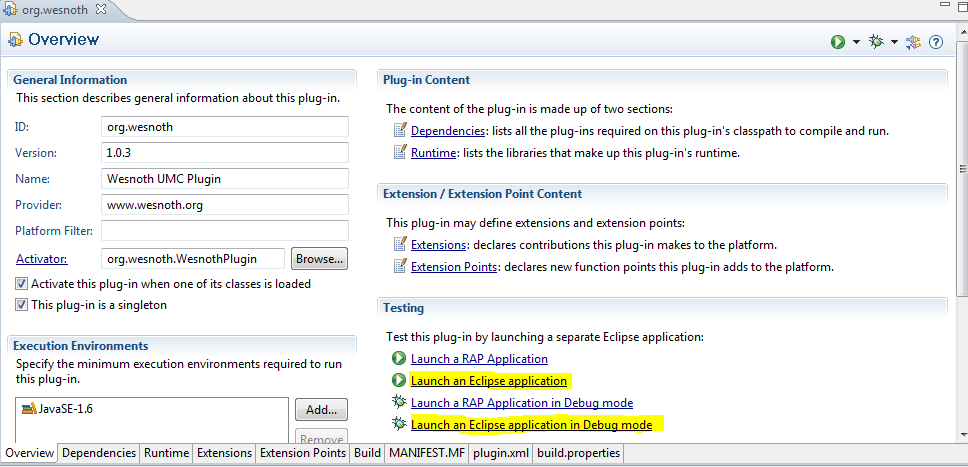
\includegraphics[width=550px]{launch_plugin.png}

\section{Frequently Asked Questions}

\end{document}
